%! Author = Wiktor Rostkowski
%! Date = 13/06/2024

\chapter{Realizacja Projektu}
\label{ch:realizacja}


\section{Faza Przedprojektowa}
\label{sec:faza-przedprojektowa}

W ramach fazy przedprojektowej zostały wykonane kluczowe dokumenty~i~analizy, które stanowią fundament dla całego projektu.\newline
\indent Na początku stworzono Kartę Projektu, która definiuje cel projektu, zakres, główne założenia oraz zasoby potrzebne do jego realizacji. 
Jest to podstawowy dokument zapewniający ogólne ramy działania~i~wytyczający kierunek dla wszystkich kolejnych działań projektowych.
\indent Następnie opracowano Dokument Założeń Wstępnych, który szczegółowo opisuje podstawowe wymagania funkcjonalne~i~niefunkcjonalne projektu. 
Ten dokument stanowi podstawę dla dalszej analizy~i~planowania działań projektowych. \newline
\indent Kolejnym kluczowym dokumentem była Specyfikacja Wymagań Systemowych (SWS), 
zawierająca szczegółowy opis wymagań systemowych, które muszą zostać spełnione~w~celu realizacji projektu. 
Celem tego etapu było udokumentowanie procesu zbierania, przetwarzania~i~analizowania wymagań oraz decyzji podjętych na podstawie tych działań.\newline
\indent Istotnym elementem tej fazy była również Analiza Rozwiązań Konkurencyjnych, która obejmowała 
przegląd~i~ocenę istniejących rozwiązań dostępnych na rynku, konkurencyjnych względem planowanego projektu.
\indent Analiza ta pozwoliła na identyfikację mocnych~i~słabych stron konkurencyjnych produktów oraz określenie unikalnych cech, które mogą 
być zaimplementowane~w~naszym projekcie.\newline
\indent Kolejnym krokiem była Analiza Aspektów Społecznych, oceniająca wpływ projektu na społeczeństwo,~w~tym 
identyfikacja potencjalnych korzyści~i~ryzyk społecznych. Analiza ta uwzględniła także kwestie etyczne~i~prawne związane z realizacją projektu. \newline
\indent Ostatnim, ale nie mniej ważnym elementem był Plan Komercjalizacji Projektu Dyplomowego, określający
 sposób na wprowadzenie projektu na rynek. Plan ten był opracowany na podstawie Business Model Canvas.\newline
Dokumentacja wykonana~w~fazie przedprojektowej stanowiła solidną podstawę dla realizacji projektu, 
zapewniając klarowne wytyczne oraz pełne zrozumienie wymagań~i~kontekstu rynkowego. Dokładne udokumentowanie procesu~i~podjętych decyzji~w~tej fazie umożliwia skuteczne zarządzanie projektem oraz minimalizowanie ryzyka związanego z jego realizacją.



\section{Przygotowanie środowiska docelowego}
\label{sec:aplikacja}

\pagebreak
\subsection{Konfiguracja Nginx}
\label{subsec:konfiguracja-nginx}
Przedstawiona poniżej konfiguracja serwera NGINX zawiera definicje kilku serwerów wirtualnych dla różnych domen i~usług.
Zamieszczono w niej szczegółowe wyjaśnienie każdego elementu konfiguracji.

\subsubsection{Główny serwer obsługujący \texttt{city-planner.budziszm.pl}}
\begin{longlisting}[language=nginx,label={lst:n1}]
server {
  server_name city-planner.budziszm.pl;

  root /var/www/city-planner.budziszm.pl/html;

  index index.html;
\end{longlisting}
\begin{itemize}
    \item \texttt{server\_name city-planner.budziszm.pl;}: Określa nazwę serwera, który obsługuje taką~konfigurację.
    \item \texttt{root /var/www/city-planner.budziszm.pl/html;}: Ustala katalog główny dla plików serwowanych przez ten serwer.
    \item \texttt{index index.html;}: Ustawia domyślny plik indeksu.
\end{itemize}

\begin{longlisting}[language=nginx,label={lst:n2}]
  location = /favicon.ico { access_log off; log_not_found off; }
\end{longlisting}
\begin{itemize}
    \item \texttt{location = /favicon.ico}: Reguła dla \texttt{favicon.ico}.
    Wyłącza logowanie dostępu oraz błędów, jeśli plik nie zostanie znaleziony.
\end{itemize}

\subsubsection{Konfiguracja gzip}
\begin{longlisting}[language=nginx,label={lst:n3}]
  gzip on;
  gzip_static on;
  gzip_types
    text/plain
    text/css
    text/js
    text/xml
    text/javascript
    application/javascript
    application/json
    application/xml
    application/rss+xml
    image/svg+xml;
  gzip_proxied no-cache no-store private expired auth;
\end{longlisting}
\begin{itemize}
    \item \texttt{gzip on;} i~\texttt{gzip\_static on;}: Włącza kompresję gzip i~kompresję statyczną.
    \item \texttt{gzip\_types}: Określa typy MIME, które mają być kompresowane.
    \item \texttt{gzip\_proxied}: Definiuje warunki, pod którymi odpowiedzi z proxy mogą być kompresowane.
\end{itemize}

\subsubsection{Konfiguracja cache dla CSS i~JS}
\begin{longlisting}[language=nginx,label={lst:n4}]
  location ~*.(css|js)$ {
    add_header Cache-Control "public, immutable, max-age=31536000";
  }
\end{longlisting}
\begin{itemize}
    \item \texttt{location ~*.(css|js)\$}: Obsługuje wszystkie pliki CSS i~JS@.
    \item \texttt{add\_header Cache-Control "public, immutable, max-age=31536000";}: Dodaje nagłówek kontrolujący cache, który umożliwia przechowywanie plików w pamięci podręcznej przez rok.
\end{itemize}

\subsubsection{Przekierowania proxy dla \texttt{/Api} i~\texttt{/confirmEmail}}
\begin{longlisting}[language=nginx,label={lst:n5}]
  location /Api {
    rewrite /Api/(.*) /$1 break;
    proxy_pass http://localhost:5000;
    proxy_redirect off;
    proxy_set_header Host $host;
  }

  location /confirmEmail {
    proxy_pass http://localhost:5000;
    proxy_redirect off;
    proxy_set_header Host $host;
  }
\end{longlisting}
\begin{itemize}
    \item \texttt{location /Api} i~\texttt{location /confirmEmail}: Przekierowują żądania na odpowiednie endpointy do lokalnego serwera działającego na porcie 5000.
\end{itemize}

\subsubsection{Obsługa plików w \texttt{/thesis}}
\begin{longlisting}[language=nginx,label={lst:n6}]
  location ~* /thesis/(.*)$ {
    root /opt/city-planner-documentation;
    rewrite /thesis/(.*) /$1.pdf break;
    add_header Content-Disposition 'inline';
    try_files $uri =404;
  }

  location /thesis {
    root /opt/city-planner-documentation;
    rewrite /thesis /thesis.pdf break;
    add_header Content-Disposition 'inline';
    try_files $uri =404;
  }
\end{longlisting}
\begin{itemize}
    \item Obsługuje dostęp do plików w katalogu \texttt{/opt/city-planner-documentation}, zmieniając ścieżki i~dodając nagłówek \texttt{Content-Disposition} do wyświetlania plików PDF w przeglądarce.
\end{itemize}

\subsubsection{Główne ustawienia dla ścieżek i~SSL}
\begin{longlisting}[language=nginx,label={lst:n7}]
  location / {
    try_files $uri$args $uri$args/ /index.html;
  }

  listen 443 ssl; # managed by Certbot
  ssl_certificate /etc/letsencrypt/live/city-planner.budziszm.pl/fullchain.pem; # managed by Certbot
  ssl_certificate_key /etc/letsencrypt/live/city-planner.budziszm.pl/privkey.pem; # managed by Certbot
  include /etc/letsencrypt/options-ssl-nginx.conf; # managed by Certbot
  ssl_dhparam /etc/letsencrypt/ssl-dhparams.pem; # managed by Certbot
\end{longlisting}
\begin{itemize}
    \item \texttt{location /}: Przekierowuje do pliku \texttt{index.html} jeśli plik lub katalog nie zostaną znalezione.
    \item \texttt{listen 443 ssl;}: Konfiguruje serwer do nasłuchiwania na porcie 443 z SSL\@.
    \item \texttt{ssl\_certificate}, \texttt{ssl\_certificate\_key}, \texttt{include}, \texttt{ssl\_dhparam}: Konfiguracja SSL przy użyciu certyfikatów Let's Encrypt.
\end{itemize}

\subsubsection{Przekierowanie HTTP do HTTPS}
\begin{longlisting}[language=nginx,label={lst:n8}]
server {
    if ($host = city-planner.budziszm.pl) {
        return 301 https://$host$request_uri;
    } # managed by Certbot

    server_name city-planner.budziszm.pl;
    listen 80;
    return 404; # managed by Certbot
}
\end{longlisting}
\begin{itemize}
    \item Przekierowuje ruch HTTP na HTTPS dla \texttt{city-planner.budziszm.pl}.
\end{itemize}

\subsubsection{Serwer obsługujący \texttt{logs.city-planner.budziszm.pl}}
\begin{longlisting}[language=nginx,label={lst:n9}]
server {
  server_name logs.city-planner.budziszm.pl;
  auth_basic           "Administrator's Area";
  auth_basic_user_file /etc/apache2/.htpasswd;
  error_log  /var/log/nginx/error.log debug;

  location / {
    proxy_pass https://localhost:18888;
    proxy_redirect off;
    proxy_http_version 1.1;
    proxy_set_header Upgrade $http_upgrade;
    proxy_set_header Connection "Upgrade";
    proxy_set_header Host $host;
  }

  listen 443 ssl; # managed by Certbot
  ssl_certificate /etc/letsencrypt/live/city-planner.budziszm.pl/fullchain.pem; # managed by Certbot
  ssl_certificate_key /etc/letsencrypt/live/city-planner.budziszm.pl/privkey.pem; # managed by Certbot
  include /etc/letsencrypt/options-ssl-nginx.conf; # managed by Certbot
  ssl_dhparam /etc/letsencrypt/ssl-dhparams.pem; # managed by Certbot
}
\end{longlisting}
\begin{itemize}
    \item Obsługuje ruch na \texttt{logs.city-planner.budziszm.pl} z podstawową autoryzacją.
    \item Przekierowuje ruch do lokalnego serwera na porcie 18888 z obsługą WebSocketów.
\end{itemize}

\subsubsection{Przekierowanie HTTP do HTTPS dla \texttt{logs.city-planner.budziszm.pl}}
\begin{longlisting}[language=nginx,label={lst:n10}]
server {
    if ($host = logs.city-planner.budziszm.pl) {
        return 301 https://$host$request_uri;
    } # managed by Certbot

    listen 80;
    server_name logs.city-planner.budziszm.pl;
    return 404; # managed by Certbot
}
\end{longlisting}
\begin{itemize}
    \item Przekierowuje ruch HTTP na HTTPS dla \texttt{logs.city-planner.budziszm.pl}.
\end{itemize}

\subsubsection{Mapowanie nagłówka \texttt{Connection} w zależności od nagłówka \texttt{Upgrade}}
\begin{longlisting}[language=nginx,label={lst:n11}]
map $http_upgrade $connection_upgrade {
  default upgrade;
  ''      close;
}
\end{longlisting}
\begin{itemize}
    \item Ustawia wartość nagłówka \texttt{Connection} w zależności od obecności nagłówka \texttt{Upgrade}.
    Umożliwia to poprawne działanie WebSocketów.
\end{itemize}

Ta konfiguracja zapewnia pełną obsługę zarówno dla serwowania statycznych stron, jak i~przekierowania ruchu do usług backendowych, zapewniając jednocześnie bezpieczeństwo przez użycie SSL i~kontrolę cache dla plików statycznych.

\subsection{Deployment backendu}
\label{subsec:deployment-backendu}
Ten skrypt Bash wykonuje kilka kroków, aby wdrożyć backend aplikacji.
Poniżej znajduje się szczegółowy opis, co robi każda jego część:

\subsubsection{Usuwanie wszystkich plików z /opt/city-planner-backend/publish}
Ten krok usuwa wszystkie pliki z katalogu \texttt{/opt/city-planner-backend/publish}, aby przygotować miejsce na nowe pliki.
\begin{longlisting}[style=shell-colored,label={lst:db1}]
+echo+ "Removing all files from /opt/city-planner-backend/publish"
+rm -Rf+ /opt/city-planner-backend/publish/*
\end{longlisting}

\subsubsection{Kopiowanie plików do /opt/city-planner-backend/publish/}
Ten krok kopiuje opublikowane pliki z katalogu \texttt{WebApi/bin/production/net8.0/linux-arm64/publish/} do \texttt{/opt/city-planner-backend/publish/}.
\begin{longlisting}[style=shell-colored,label={lst:db2}]
+echo+ "Copying publish files to /opt/city-planner-backend/publish/"
+cp+ WebApi/bin/production/net8.0/linux-arm64/publish/* /opt/city-planner-backend/publish/
\end{longlisting}

\subsubsection{Przygotowanie pliku usługi SystemD}
Ten krok tworzy nowy plik usługi SystemD dla backendu aplikacji.
Plik usługi zawiera konfigurację dla SystemD, w tym opis, zależności, ustawienia serwisu i~polecenie uruchomienia.

\begin{longlisting}[style=shell-colored,label={lst:db3}]
+echo+ "Preparing SystemD service file"
+rm -f+ /etc/systemd/system/city-planner-backend.service
+cat+ <<EOT >> /etc/systemd/system/city-planner-backend.service
[Unit]
Description=City planner backend
After=network.target
StartLimitIntervalSec=0

[Service]
Type=simple
Restart=always
RestartSec=1
User=ubuntu
EnvironmentFile=/opt/city-planner-backend/environment.conf
WorkingDirectory=/opt/city-planner-backend/publish
ExecStart=/opt/city-planner-backend/publish/WebApi

[Install]
WantedBy=multi-user.target
EOT
\end{longlisting}

\subsubsection{Włączanie pliku usługi SystemD}
Ten krok włącza nowo utworzony plik usługi SystemD, aby uruchamiał się automatycznie przy starcie systemu.
\begin{longlisting}[style=shell-colored,label={lst:db4}]
+echo+ "Enabling SystemD service file"
+systemctl enable+ city-planner-backend
\end{longlisting}

\subsubsection{Restartowanie usługi SystemD}
Ten krok restartuje usługę SystemD, aby zastosować nowe ustawienia i~uruchomić backend aplikacji.
\begin{longlisting}[style=shell-colored,label={lst:db5}]
+echo+ "Restarting SystemD service file"
+systemctl restart+ city-planner-backend
\end{longlisting}

\subsubsection{Zakończenie wdrożenia backendu}
Ten krok wyświetla komunikat informujący o zakończeniu wdrożenia backendu.
\begin{longlisting}[style=shell-colored,label={lst:db6}]
+echo+ "Backend deployment done"
\end{longlisting}

\subsubsection{Całość kodu}
\begin{longlisting}[style=shell-colored,label={lst:db7}]
#!/bin/bash

+echo+ "Removing all files from /opt/city-planner-backend/publish"
+rm -Rf+ /opt/city-planner-backend/publish/*

+echo+ "Copying publish files to /opt/city-planner-backend/publish/"
+cp+ WebApi/bin/production/net8.0/linux-arm64/publish/* /opt/city-planner-backend/publish/
+echo+ "Preparing SystemD service file"
+rm -f+ /etc/systemd/system/city-planner-backend.service
+cat+ <<EOT >> /etc/systemd/system/city-planner-backend.service
[Unit]
Description=City planner backend
After=network.target
StartLimitIntervalSec=0

[Service]
Type=simple
Restart=always
RestartSec=1
User=ubuntu
EnvironmentFile=/opt/city-planner-backend/environment.conf
WorkingDirectory=/opt/city-planner-backend/publish
ExecStart=/opt/city-planner-backend/publish/WebApi

[Install]
WantedBy=multi-user.target
EOT

+echo+ "Enabling SystemD service file"
+systemctl enable+ city-planner-backend
+echo+ "Restarting SystemD service file"
+systemctl restart+ city-planner-backend

+echo+ "Backend deployment done"
\end{longlisting}

\subsection{Deployment frontendu}
Ten skrypt Bash wykonuje kilka kroków, aby wdrożyć frontend aplikacji.
Poniżej znajduje się szczegółowy opis, co robi każda jego część:

\subsubsection{Usuwanie wszystkich plików z \newline
/var/www/city-planner.budziszm.pl/html}
Ten krok usuwa wszystkie pliki z katalogu \texttt{/var/www/city-planner.budziszm.pl/html}, aby przygotować miejsce na nowe pliki.
\begin{longlisting}[style=shell-colored]
+echo+ "Removing all files from /var/www/city-planner.budziszm.pl/html"
+rm -Rf+ /var/www/city-planner.budziszm.pl/html/*
\end{longlisting}

\subsubsection{Kopiowanie plików do /var/www/city-planner.budziszm.pl/html/}
Ten krok kopiuje pliki z katalogu \texttt{dist/frontend/browser/} \newline
do \texttt{/var/www/city-planner.budziszm.pl/html/}.
\begin{longlisting}[style=shell-colored]
+echo+ "Copying dist files to /var/www/city-planner.budziszm.pl/html/"
+cp -r+ dist/frontend/browser/* /var/www/city-planner.budziszm.pl/html/
\end{longlisting}

\subsubsection{Zakończenie wdrożenia frontendu}
Ten krok wyświetla komunikat informujący o zakończeniu wdrożenia frontendu.
\begin{longlisting}[style=shell-colored]
+echo+ "Frontend deployment done"
\end{longlisting}

\subsubsection{Całość kodu}
\begin{longlisting}[style=shell-colored]
#!/bin/bash

+echo+ "Removing all files from /var/www/city-planner.budziszm.pl/html"
+rm -Rf+ /var/www/city-planner.budziszm.pl/html/*

+echo+ "Copying dist files to /var/www/city-planner.budziszm.pl/html/"
+cp -r+ dist/frontend/browser/* /var/www/city-planner.budziszm.pl/html/

+echo+ "Frontend deployment done"
\end{longlisting}

\section{Specyfikacja API}
Do implementacji API został użyty framework ASP.NET 8, który umożliwia tworzenie wydajnych i~skalowalnych aplikacji webowych. Do zarządzania warstwą dostępu do danych i~mapowania obiektowo-relacyjnego (ORM) zastosowano Entity Framework, w połączeniu z biblioteką Npgsql, która pozwala na efektywną współpracę z bazą danych PostgreSQL\@.
Dzięki temu rozwiązaniu możliwe było stworzenie solidnej i~wydajnej aplikacji z wykorzystaniem nowoczesnych technologii .NET, zapewniając jednocześnie łatwość w zarządzaniu danymi i~wysoką kompatybilność z relacyjnymi bazami danych.

W trakcie prac do prezentacji dokumentacji endpointów użyto Swaggera i~ReDoca.

\begin{figure}[H]
\centering
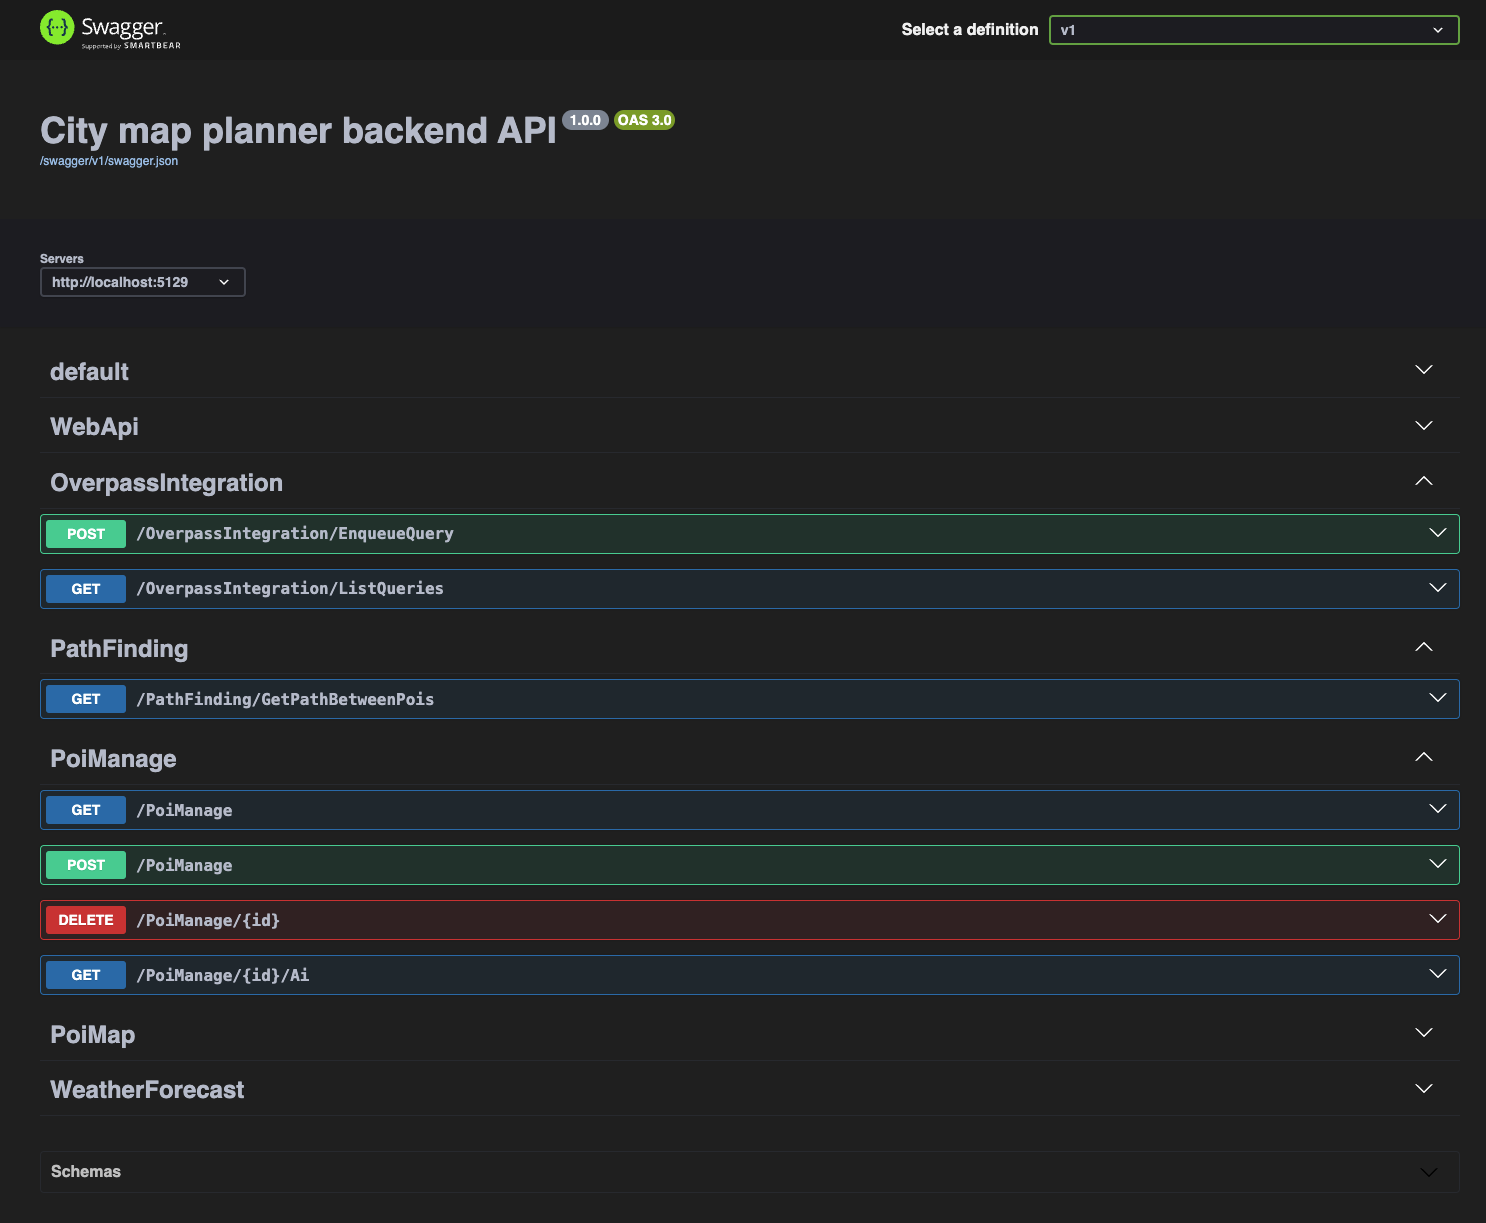
\includegraphics[width=1\textwidth]{attachments/swagger}
\caption{Dokumentacji API w programie Swagger}
\label{fig:figure}
\end{figure}

\begin{figure}[H]
\centering

\includegraphics[width=1\textwidth]{attachments/redoc}
\caption{Dokumentacji API w programie ReDoc}
\label{fig:figure}
\end{figure}

Poniżej przedstawiono specyfikację dostępnych punktów końcowych:

\subsection{Autoryzacja i~zarządzanie użytkownikami}
\subsubsection{\lstinline[language=http]{POST /register}}
Rejestracja nowego użytkownika. \\
\textbf{Request body:}
\begin{lstlisting}[language=json]
{
  "email": "string",
  "password": "string"
}
\end{lstlisting}
\textbf{Responses:}
\begin{itemize}
    \item 200: Rejestracja powiodła się.
    \item 400: Błąd walidacji danych.
\begin{lstlisting}[language=json]
{
  "type": "string",
  "title": "string",
  "status": 0,
  "detail": "string",
  "instance": "string",
  "errors": {
    "additionalProp1": [
      "string"
    ],
    "additionalProp2": [
      "string"
    ],
    "additionalProp3": [
      "string"
    ]
  }
}
\end{lstlisting}
\end{itemize}

\subsubsection{\lstinline[language=http]{POST /login}}
Logowanie użytkownika. \\
\textbf{Query parameters:}
\begin{itemize}
    \item \texttt{useCookies} (boolean, opcjonalny)
    \item \texttt{useSessionCookies} (boolean, opcjonalny)
\end{itemize}
\textbf{Request body:}
\begin{lstlisting}[language=json]
{
  "email": "string",
  "password": "string",
  "twoFactorCode": "string",
  "twoFactorRecoveryCode": "string"
}
\end{lstlisting}
\textbf{Responses:}
\begin{itemize}
    \item 200:
\begin{lstlisting}[language=json]
{
  "tokenType": "string",
  "accessToken": "string",
  "expiresIn": 0,
  "refreshToken": "string"
}
\end{lstlisting}
\end{itemize}

\subsubsection{\lstinline[language=http]{POST /refresh}}
Odświeżenie tokenu autoryzacyjnego. \\
\textbf{Request body:}
\begin{lstlisting}[language=json]
{
  "refreshToken": "string"
}
\end{lstlisting}
\textbf{Responses:}
\begin{itemize}
    \item 200:
\begin{lstlisting}[language=json]
{
  "tokenType": "string",
  "accessToken": "string",
  "expiresIn": 0,
  "refreshToken": "string"
}
\end{lstlisting}
\end{itemize}

\subsubsection{\lstinline[language=http]{GET /confirmEmail}}
Potwierdzenie adresu email. \\
\textbf{Query parameters:}
\begin{itemize}
    \item \texttt{userId} (string, opcjonalny)
    \item \texttt{code} (string, opcjonalny)
    \item \texttt{changedEmail} (string, opcjonalny)
\end{itemize}
\textbf{Responses:}
\begin{itemize}
    \item 200: Potwierdzenie zakończone sukcesem.
\end{itemize}

\subsubsection{\lstinline[language=http]{POST /resendConfirmationEmail}}
Ponowne wysłanie emaila z potwierdzeniem. \\
\textbf{Request body:}
\begin{lstlisting}[language=json]
{
  "email": "string"
}
\end{lstlisting}
\textbf{Responses:}
\begin{itemize}
    \item 200: Email z potwierdzeniem wysłany ponownie.
\end{itemize}

\subsubsection{\lstinline[language=http]{POST /forgotPassword}}
Przypomnienie hasła. \\
\textbf{Request body:}
\begin{lstlisting}[language=json]
{
  "email": "string"
}
\end{lstlisting}
\textbf{Responses:}
\begin{itemize}
    \item 200: Email z instrukcjami wysłany.
    \item 400:
\begin{lstlisting}[language=json]
{
  "type": "string",
  "title": "string",
  "status": 0,
  "detail": "string",
  "instance": "string",
  "errors": {
    "additionalProp1": [
      "string"
    ],
    "additionalProp2": [
      "string"
    ],
    "additionalProp3": [
      "string"
    ]
  }
}
\end{lstlisting}
\end{itemize}

\subsubsection{\lstinline[language=http]{POST /resetPassword}}
Resetowanie hasła. \\
\textbf{Request body:}
\begin{lstlisting}[language=json]
{
  "email": "string",
  "resetCode": "string",
  "newPassword": "string"
}
\end{lstlisting}
\textbf{Responses:}
\begin{itemize}
    \item 200: Hasło zresetowane.
    \item 400:
\begin{lstlisting}[language=json]
{
  "type": "string",
  "title": "string",
  "status": 0,
  "detail": "string",
  "instance": "string",
  "errors": {
    "additionalProp1": [
      "string"
    ],
    "additionalProp2": [
      "string"
    ],
    "additionalProp3": [
      "string"
    ]
  }
}
\end{lstlisting}
\end{itemize}

\subsubsection{\lstinline[language=http]{POST /manage/2fa}}
Zarządzanie dwuskładnikowym uwierzytelnianiem (2FA). \\
\textbf{Request body:}
\begin{lstlisting}[language=json]
{
  "enable": true,
  "twoFactorCode": "string",
  "resetSharedKey": true,
  "resetRecoveryCodes": true,
  "forgetMachine": true
}
\end{lstlisting}
\textbf{Responses:}
\begin{itemize}
    \item 200:
\begin{lstlisting}[language=json]
{
  "sharedKey": "string",
  "recoveryCodesLeft": 0,
  "recoveryCodes": [
    "string"
  ],
  "isTwoFactorEnabled": true,
  "isMachineRemembered": true
}
\end{lstlisting}
    \item 400:
\begin{lstlisting}[language=json]
{
  "type": "string",
  "title": "string",
  "status": 0,
  "detail": "string",
  "instance": "string",
  "errors": {
    "additionalProp1": [
      "string"
    ],
    "additionalProp2": [
      "string"
    ],
    "additionalProp3": [
      "string"
    ]
  }
}
\end{lstlisting}
    \item 404: Nie znaleziono zasobu.
\end{itemize}

\subsubsection{\lstinline[language=http]{GET /manage/info}}
Pobranie informacji o koncie. \\
\textbf{Responses:}
\begin{itemize}
    \item 200:
\begin{lstlisting}[language=json]
{
  "email": "string",
  "isEmailConfirmed": true
}
\end{lstlisting}
    \item 400:
\begin{lstlisting}[language=json]
{
  "type": "string",
  "title": "string",
  "status": 0,
  "detail": "string",
  "instance": "string",
  "errors": {
    "additionalProp1": [
      "string"
    ],
    "additionalProp2": [
      "string"
    ],
    "additionalProp3": [
      "string"
    ]
  }
}
\end{lstlisting}
    \item 404: Nie znaleziono zasobu.
\end{itemize}

\subsubsection{\lstinline[language=http]{POST /manage/info}}
Aktualizacja informacji o koncie. \\
\textbf{Request body:}
\begin{lstlisting}[language=json]
{
  "newEmail": "string",
  "newPassword": "string",
  "oldPassword": "string"
}
\end{lstlisting}
\textbf{Responses:}
\begin{itemize}
    \item 200:
\begin{lstlisting}[language=json]
{
  "email": "string",
  "isEmailConfirmed": true
}
\end{lstlisting}
    \item 400:
\begin{lstlisting}[language=json]
{
  "type": "string",
  "title": "string",
  "status": 0,
  "detail": "string",
  "instance": "string",
  "errors": {
    "additionalProp1": [
      "string"
    ],
    "additionalProp2": [
      "string"
    ],
    "additionalProp3": [
      "string"
    ]
  }
}
\end{lstlisting}
    \item 404: Nie znaleziono zasobu.
\end{itemize}

\subsubsection{\lstinline[language=http]{POST /logout}}
Wylogowanie użytkownika. \\
\textbf{Request body:} Pusty JSON \\
\textbf{Responses:}
\begin{itemize}
    \item 200: Wylogowanie zakończone sukcesem.
\end{itemize}

\subsubsection{\lstinline[language=http]{GET /exists}}
Sprawdzenie czy email istnieje w systemie. \\
\textbf{Query parameters:}
\begin{itemize}
    \item \texttt{email} (string, wymagany)
\end{itemize}
\textbf{Responses:}
\begin{itemize}
    \item 200: Email istnieje.
\end{itemize}

\subsubsection{\lstinline[language=http]{POST /deleteMe}}
Usunięcie konta użytkownika. \\
\textbf{Responses:}
\begin{itemize}
    \item 200: Konto usunięte.
\end{itemize}

\subsection{Integracja z Overpass}

\subsubsection{\lstinline[language=http]{POST /OverpassIntegration/EnqueueQuery}}
Kolejkowanie zapytania Overpass. \\
\textbf{Responses:}
\begin{itemize}
    \item 200: Zapytanie dodane do kolejki.
\end{itemize}

\subsubsection{\lstinline[language=http]{GET /OverpassIntegration/ListQueries}}
Pobranie listy zapytań Overpass. \\
\textbf{Responses:}
\begin{lstlisting}[language=json]
[
  "string"
]
\end{lstlisting}
\begin{itemize}
    \item 401: Nieautoryzowany dostęp.
\end{itemize}

\subsection{Zarządzanie Punktami POI}

\subsubsection{\lstinline[language=http]{GET /PoiManage}}
Pobranie listy punktów POI. \\
\textbf{Responses:}
\begin{lstlisting}[language=json]
[
  {
    "id": 0,
    "name": "string",
    "description": "string",
    "modified": "2023-01-01T00:00:00Z",
    "businessHoursPageUrl": "string",
    "businessHoursPageXPath": "string",
    "businessHoursPageModified": "2023-01-01T00:00:00Z",
    "holidaysPageUrl": "string",
    "holidaysPageXPath": "string",
    "holidaysPageModified": "2023-01-01T00:00:00Z",
    "entrances": [
      {
        "osmNodeId": 0,
        "name": "string",
        "description": "string"
      }
    ],
    "images": [
      {
        "fullSrc": "string",
        "iconSrc": "string",
        "attribution": "string"
      }
    ],
    "preferredWmoCodes": [
      0
    ],
    "preferredSightseeingTime": "string",
    "businessTimes": [
      {
        "effectiveFrom": "2023-01-01T00:00:00Z",
        "effectiveTo": "2023-01-01T00:00:00Z",
        "effectiveDays": [
          0
        ],
        "timeFrom": "00:00:00",
        "timeTo": "00:00:00",
        "state": 0
      }
    ]
  }
]
\end{lstlisting}

\subsubsection{\lstinline[language=http]{POST /PoiManage}}
Dodanie lub aktualizacja punktu POI. \\
\textbf{Request body:}
\begin{lstlisting}[language=json]
{
  "id": 0,
  "name": "string",
  "description": "string",
  "modified": "2023-01-01T00:00:00Z",
  "businessHoursPageUrl": "string",
  "businessHoursPageXPath": "string",
  "businessHoursPageModified": "2023-01-01T00:00:00Z",
  "holidaysPageUrl": "string",
  "holidaysPageXPath": "string",
  "holidaysPageModified": "2023-01-01T00:00:00Z",
  "entrances": [
    {
      "osmNodeId": 0,
      "name": "string",
      "description": "string"
    }
  ],
  "images": [
    {
      "fullSrc": "string",
      "iconSrc": "string",
      "attribution": "string"
    }
  ],
  "preferredWmoCodes": [
    0
  ],
  "preferredSightseeingTime": "string",
  "businessTimes": [
    {
      "effectiveFrom": "2023-01-01T00:00:00Z",
      "effectiveTo": "2023-01-01T00:00:00Z",
      "effectiveDays": [
        0
      ],
      "timeFrom": "00:00:00",
      "timeTo": "00:00:00",
      "state": 0
    }
  ]
}
\end{lstlisting}
\textbf{Responses:}
\begin{lstlisting}[language=json]
{
  "id": 0,
  "name": "string",
  "description": "string",
  "modified": "2023-01-01T00:00:00Z",
  "businessHoursPageUrl": "string",
  "businessHoursPageXPath": "string",
  "businessHoursPageModified": "2023-01-01T00:00:00Z",
  "holidaysPageUrl": "string",
  "holidaysPageXPath": "string",
  "holidaysPageModified": "2023-01-01T00:00:00Z",
  "entrances": [
    {
      "osmNodeId": 0,
      "name": "string",
      "description": "string"
    }
  ],
  "images": [
    {
      "fullSrc": "string",
      "iconSrc": "string",
      "attribution": "string"
    }
  ],
  "preferredWmoCodes": [
    0
  ],
  "preferredSightseeingTime": "string",
  "businessTimes": [
    {
      "effectiveFrom": "2023-01-01T00:00:00Z",
      "effectiveTo": "2023-01-01T00:00:00Z",
      "effectiveDays": [
        0
      ],
      "timeFrom": "00:00:00",
      "timeTo": "00:00:00",
      "state": 0
    }
  ]
}
\end{lstlisting}

\subsubsection{\lstinline[language=http]{DELETE /PoiManage/\{id\}}}
Usunięcie punktu POI. \\
\textbf{Path parameters:}
\begin{itemize}
    \item \texttt{id} (integer, wymagany)
\end{itemize}
\textbf{Responses:}
\begin{itemize}
    \item 200: Punkt POI usunięty.
\end{itemize}

\subsubsection{\lstinline[language=http]{GET /PoiManage/\{id\}/Ai}}
Pobranie informacji AI dla punktu POI. \\
\textbf{Path parameters:}
\begin{itemize}
    \item \texttt{id} (integer, wymagany)
\end{itemize}
\textbf{Responses:}
\begin{lstlisting}[language=json]
[
  {
    "effectiveFrom": "2023-01-01T00:00:00Z",
    "effectiveTo": "2023-01-01T00:00:00Z",
    "effectiveDays": [
      0
    ],
    "timeFrom": "00:00:00",
    "timeTo": "00:00:00",
    "state": 0
  }
]
\end{lstlisting}

\subsection{Mapowanie Punktów POI}

\subsubsection{\lstinline[language=http]{GET /PoiMap/List}}
Lista punktów POI na mapie. \\
\textbf{Responses:}
\begin{lstlisting}[language=json]
[
  {
    "id": 0,
    "map": {
      "label": "string",
      "iconSrc": "string",
      "lat": 0,
      "lon": 0
    },
    "details": {
      "bannerSrc": "string",
      "title": "string",
      "description": "string"
    },
    "preferredSightseeingTime": "string",
    "businessHours": [
      {
        "effectiveFrom": "2023-01-01T00:00:00Z",
        "effectiveTo": "2023-01-01T00:00:00Z",
        "effectiveDays": [
          0
        ],
        "timeFrom": "00:00:00",
        "timeTo": "00:00:00",
        "state": 0
      }
    ]
  }
]
\end{lstlisting}

\subsubsection{\lstinline[language=http]{GET /WeatherStatus/List}}
Pobranie prognozy pogody z klienta pogodowego OpenMeteo\\
\textbf{Responses:}
\begin{lstlisting}[language=json]
  [
    {
      "time": "2024-06-15T11:42:38.897Z",
      "weathercode": 0,
      "temperature2M": 0
    }
  ]
\end{lstlisting}

\subsubsection{\lstinline[language=http]{GET /WeatherForecast}}
Pobranie prognozy pogody dla testu działania aplikacji\\
\textbf{Responses:}
\begin{lstlisting}[language=json]
  [
    {
      "date": "2024-06-15",
      "temperatureC": 0,
      "temperatureF": 0,
      "summary": "string"
    }
  ]
\end{lstlisting}

\section{Baza danych}
Baza danych została podzielona na dwa schematy: \texttt{data} oraz \texttt{user\_data}, aby lepiej zarządzać różnymi rodzajami informacji.
Schemat \texttt{data} zawiera informacje o atrakcjach turystycznych oraz mapie miasta, które są dostępne publicznie.
Dane te mogą obejmować opisy zabytków, godziny otwarcia, lokalizacje na mapie oraz inne informacje przydatne dla turystów.\newline
Z kolei schemat \texttt{user\_data} przechowuje tylko dane logowania oraz uprawnienia użytkowników.
Taki podział pozwala na lepsze zabezpieczenie danych użytkowników, usprawnienie zarządzania bazą danych oraz łatwiejsze stosowanie różnych poziomów dostępu i~kontroli nad danymi.
Tabele posiadają różnorodne klucze obce, które zapewniają integralność danych poprzez powiązania między tabelami oraz mechanizm kaskadowego usuwania.

\subsection{Schemat \texttt{user\_data}}

\begin{figure}[H]
\centering
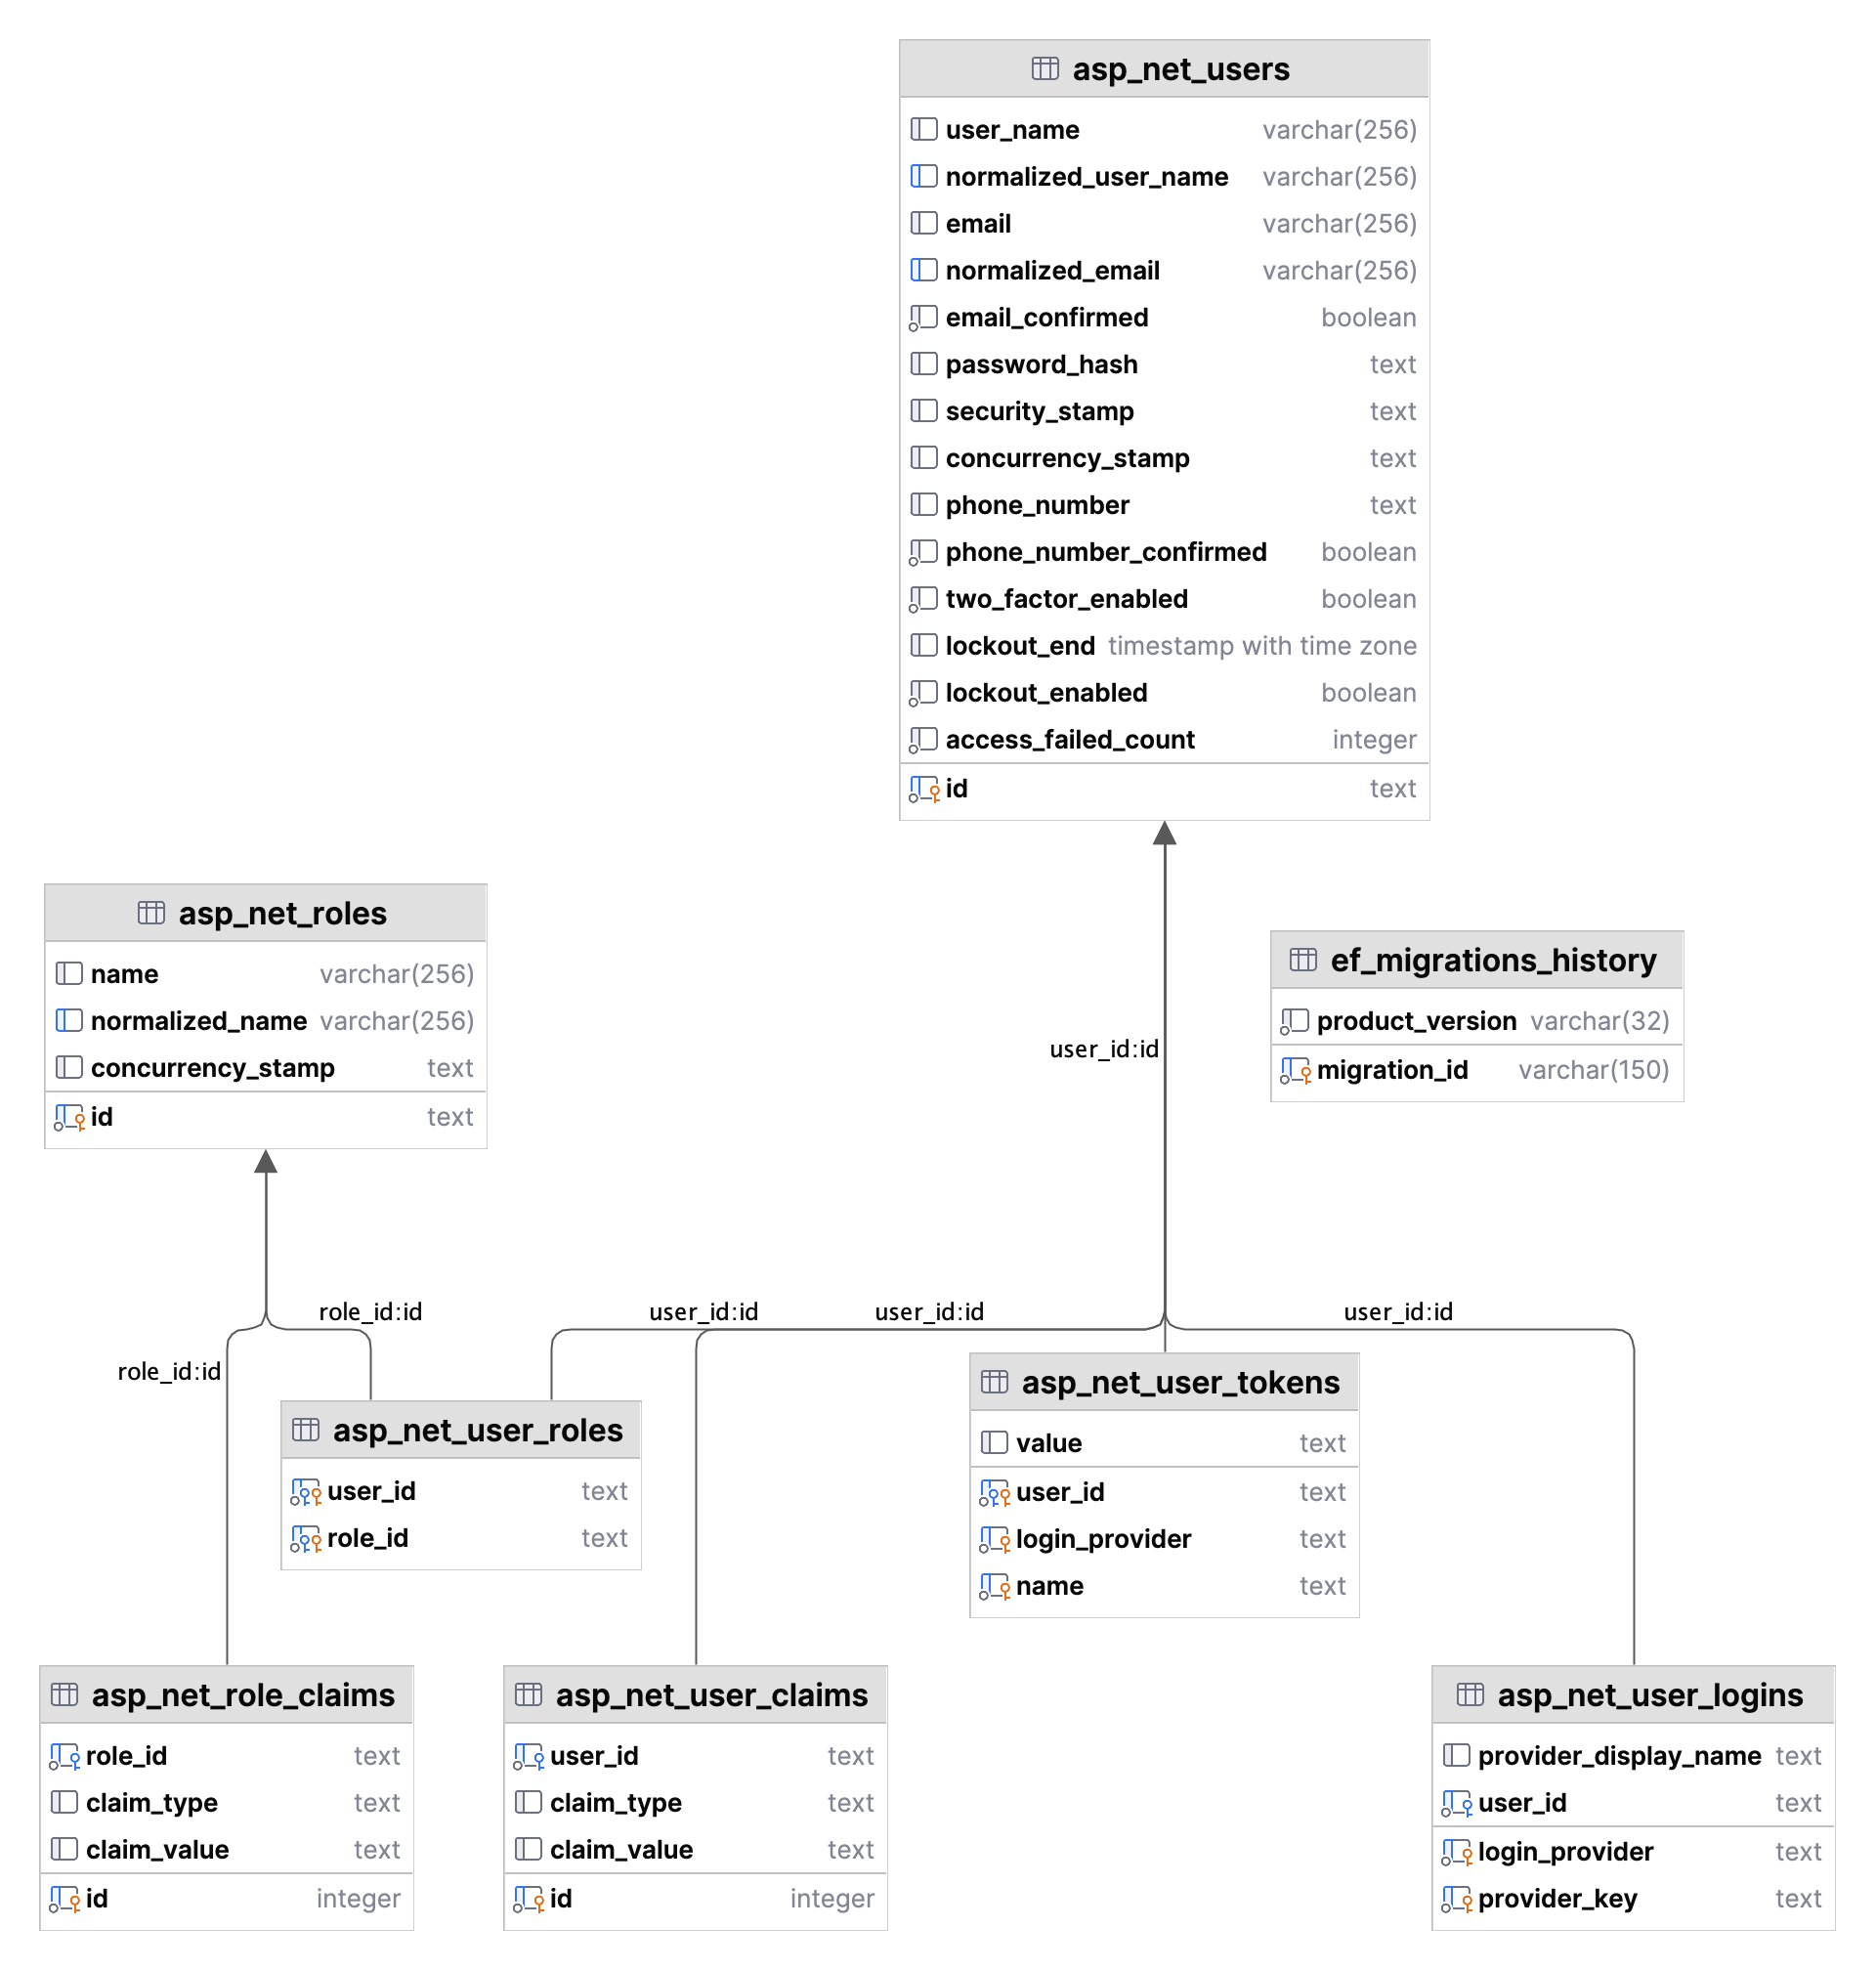
\includegraphics[width=1\textwidth]{attachments/user_data}
\caption{Diagram ERD schematu user\_data}
\label{fig:figure}
\end{figure}

\subsubsection{Tabela \keyword{ef\_migrations\_history}}
Tabela przechowuje historię migracji bazy danych.
\begin{itemize}
    \item \keyword{migration\_id}: \keyword{varchar(150)}, klucz główny, nie może być \keyword{NULL}
    \item \keyword{product\_version}: \keyword{varchar(32)}, nie może być \keyword{NULL}
\end{itemize}

\subsubsection{Tabela \keyword{asp\_net\_roles}}
Tabela przechowuje informacje o rolach użytkowników.
\begin{itemize}
    \item \keyword{id}: \keyword{text}, klucz główny, nie może być \keyword{NULL}
    \item \keyword{name}: \keyword{varchar(256)}
    \item \keyword{normalized\_name}: \keyword{varchar(256)}
    \item \keyword{concurrency\_stamp}: \keyword{text}
\end{itemize}
Indeksy:
\begin{itemize}
    \item \keyword{RoleNameIndex} na kolumnie \keyword{normalized\_name} (unikatowy)
\end{itemize}

\subsubsection{Tabela \keyword{asp\_net\_users}}
Tabela przechowuje informacje o użytkownikach.
\begin{itemize}
    \item \keyword{id}: \keyword{text}, klucz główny, nie może być \keyword{NULL}
    \item \keyword{user\_name}: \keyword{varchar(256)}
    \item \keyword{normalized\_user\_name}: \keyword{varchar(256)}
    \item \keyword{email}: \keyword{varchar(256)}
    \item \keyword{normalized\_email}: \keyword{varchar(256)}
    \item \keyword{email\_confirmed}: \keyword{boolean}, nie może być \keyword{NULL}
    \item \keyword{password\_hash}: \keyword{text}
    \item \keyword{security\_stamp}: \keyword{text}
    \item \keyword{concurrency\_stamp}: \keyword{text}
    \item \keyword{phone\_number}: \keyword{text}
    \item \keyword{phone\_number\_confirmed}: \keyword{boolean}, nie może być \keyword{NULL}
    \item \keyword{two\_factor\_enabled}: \keyword{boolean}, nie może być \keyword{NULL}
    \item \keyword{lockout\_end}: \keyword{timestamp with time zone}
    \item \keyword{lockout\_enabled}: \keyword{boolean}, nie może być \keyword{NULL}
    \item \keyword{access\_failed\_count}: \keyword{integer}, nie może być \keyword{NULL}
\end{itemize}
Indeksy:
\begin{itemize}
    \item \keyword{EmailIndex} na kolumnie \keyword{normalized\_email}
    \item \keyword{UserNameIndex} na kolumnie \keyword{normalized\_user\_name} (unikatowy)
\end{itemize}

\subsubsection{Tabela \keyword{asp\_net\_role\_claims}}
Tabela przechowuje informacje o roszczeniach przypisanych do ról.
\begin{itemize}
    \item \keyword{id}: \keyword{integer}, generowany automatycznie, klucz główny
    \item \keyword{role\_id}: \keyword{text}, nie może być \keyword{NULL}, klucz obcy od \keyword{asp\_net\_roles}, kaskadowe usuwanie
    \item \keyword{claim\_type}: \keyword{text}
    \item \keyword{claim\_value}: \keyword{text}
\end{itemize}
Indeksy:
\begin{itemize}
    \item \keyword{ix\_asp\_net\_role\_claims\_role\_id} na kolumnie \keyword{role\_id}
\end{itemize}

\subsubsection{Tabela \keyword{asp\_net\_user\_claims}}
Tabela przechowuje informacje o roszczeniach przypisanych do użytkowników.
\begin{itemize}
    \item \keyword{id}: \keyword{integer}, generowany automatycznie, klucz główny
    \item \keyword{user\_id}: \keyword{text}, nie może być \keyword{NULL}, klucz obcy od \keyword{asp\_net\_users}, kaskadowe usuwanie
    \item \keyword{claim\_type}: \keyword{text}
    \item \keyword{claim\_value}: \keyword{text}
\end{itemize}
Indeksy:
\begin{itemize}
    \item \keyword{ix\_asp\_net\_user\_claims\_user\_id} na kolumnie \keyword{user\_id}
\end{itemize}

\subsubsection{Tabela \keyword{asp\_net\_user\_logins}}
Tabela przechowuje informacje o logowaniach użytkowników.
\begin{itemize}
    \item \keyword{login\_provider}: \keyword{text}, nie może być \keyword{NULL}
    \item \keyword{provider\_key}: \keyword{text}, nie może być \keyword{NULL}
    \item \keyword{provider\_display\_name}: \keyword{text}
    \item \keyword{user\_id}: \keyword{text}, nie może być \keyword{NULL}, klucz obcy od \keyword{asp\_net\_users}, kaskadowe usuwanie
    \item Klucz główny: (\keyword{login\_provider}, \keyword{provider\_key})
\end{itemize}
Indeksy:
\begin{itemize}
    \item \keyword{ix\_asp\_net\_user\_logins\_user\_id} na kolumnie \keyword{user\_id}
\end{itemize}

\subsubsection{Tabela \keyword{asp\_net\_user\_roles}}
Tabela przechowuje informacje o przypisaniu ról do użytkowników.
\begin{itemize}
    \item \keyword{user\_id}: \keyword{text}, nie może być \keyword{NULL}, klucz obcy od \keyword{asp\_net\_users}, kaskadowe usuwanie
    \item \keyword{role\_id}: \keyword{text}, nie może być \keyword{NULL}, klucz obcy od \keyword{asp\_net\_roles}, kaskadowe usuwanie
    \item Klucz główny: (\keyword{user\_id}, \keyword{role\_id})
\end{itemize}
Indeksy:
\begin{itemize}
    \item \keyword{ix\_asp\_net\_user\_roles\_role\_id} na kolumnie \keyword{role\_id}
\end{itemize}

\subsubsection{Tabela \keyword{asp\_net\_user\_tokens}}
Tabela przechowuje informacje o tokenach użytkowników.
\begin{itemize}
    \item \keyword{user\_id}: \keyword{text}, nie może być \keyword{NULL}, klucz obcy od \keyword{asp\_net\_users}, kaskadowe usuwanie
    \item \keyword{login\_provider}: \keyword{text}, nie może być \keyword{NULL}
    \item \keyword{name}: \keyword{text}, nie może być \keyword{NULL}
    \item \keyword{value}: \keyword{text}
    \item Klucz główny: (\keyword{user\_id}, \keyword{login\_provider}, \keyword{name})
\end{itemize}

\subsection{Schemat \texttt{data}}

\begin{figure}[H]
\centering
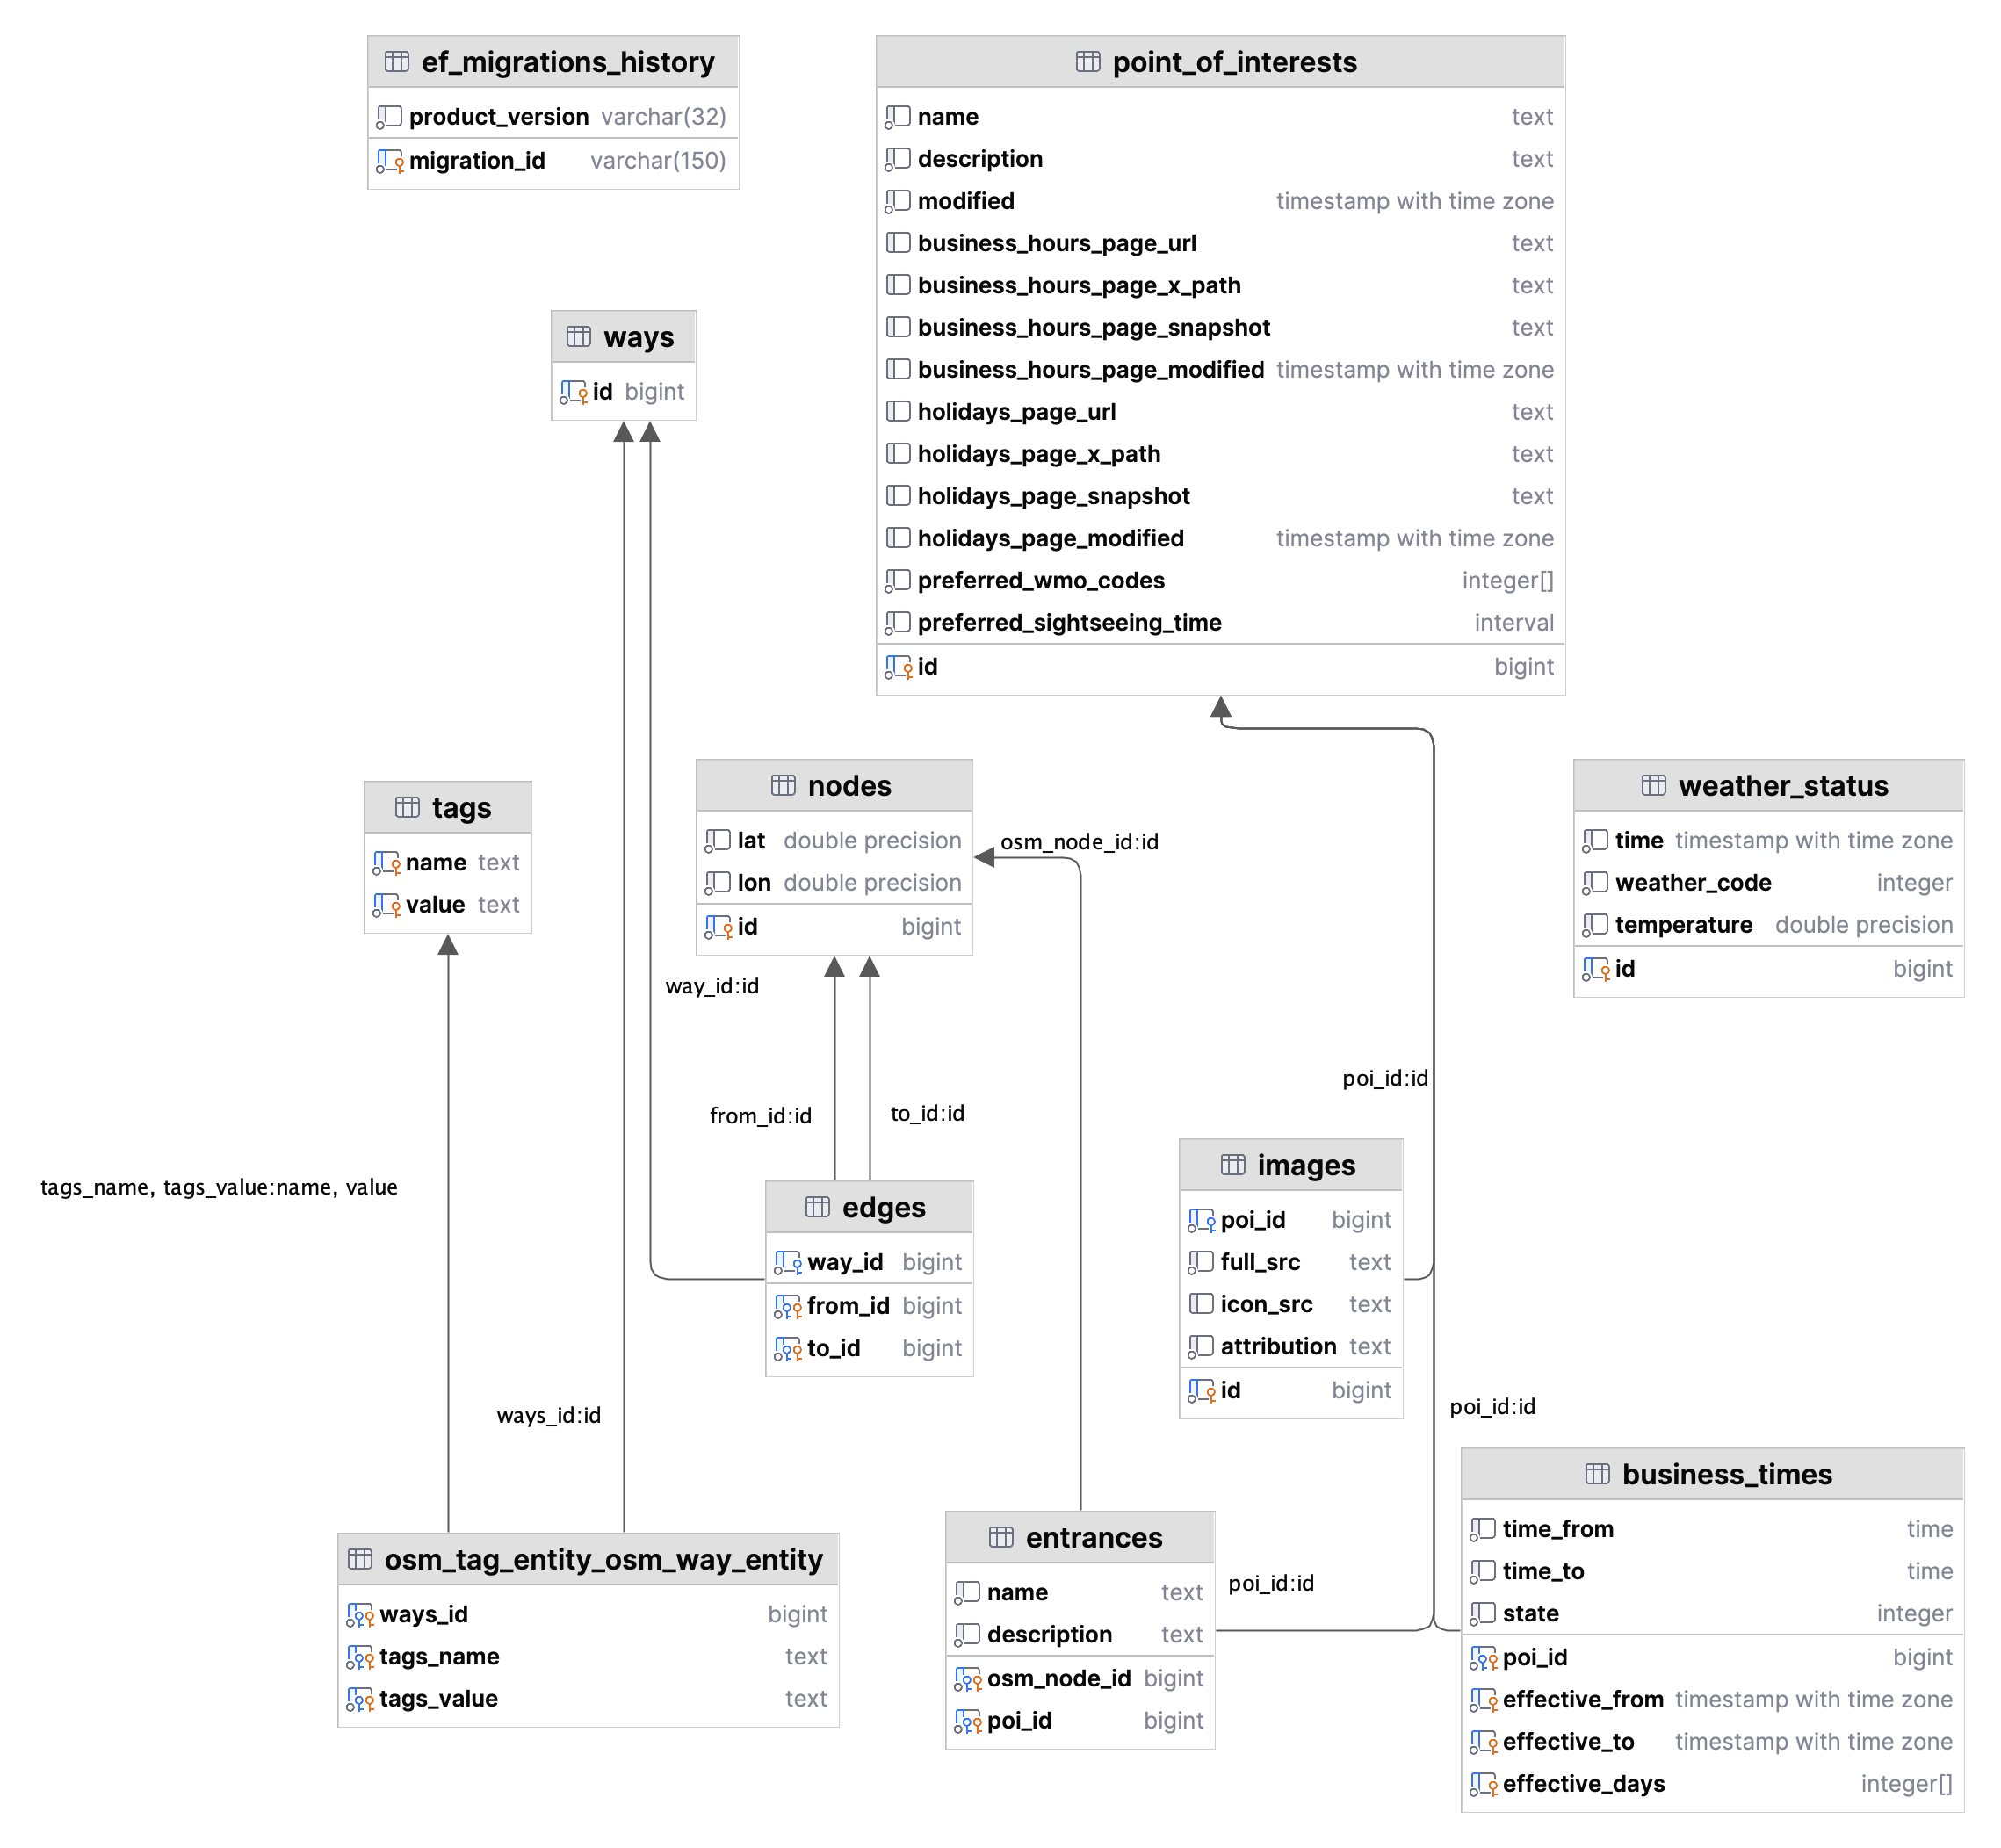
\includegraphics[width=1\textwidth]{attachments/data}
\caption{Diagram ERD schematu data}
\label{fig:figure}
\end{figure}

\subsubsection{Tabela \keyword{ef\_migrations\_history}}
Tabela przechowuje historię migracji bazy danych.
\begin{itemize}
    \item \keyword{migration\_id}: \keyword{varchar(150)}, klucz główny, nie może być \keyword{NULL}
    \item \keyword{product\_version}: \keyword{varchar(32)}, nie może być \keyword{NULL}
\end{itemize}

\subsubsection{Tabela \keyword{nodes}}
Tabela przechowuje informacje o węzłach, w tym ich identyfikator oraz współrzędne geograficzne.
\begin{itemize}
    \item \keyword{id}: \keyword{bigint}, klucz główny, nie może być \keyword{NULL}
    \item \keyword{lat}: \keyword{double precision}, nie może być \keyword{NULL}
    \item \keyword{lon}: \keyword{double precision}, nie może być \keyword{NULL}
\end{itemize}

\subsubsection{Tabela \keyword{point\_of\_interests}}
Tabela przechowuje informacje o punktach zainteresowania, takich jak nazwa, opis oraz godziny otwarcia.
\begin{itemize}
    \item \keyword{id}: \keyword{bigint}, generowany automatycznie, klucz główny
    \item \keyword{name}: \keyword{text}, nie może być \keyword{NULL}
    \item \keyword{description}: \keyword{text}, nie może być \keyword{NULL}
    \item \keyword{modified}: \keyword{timestamp with time zone}, nie może być \keyword{NULL}
    \item \keyword{business\_hours\_page\_url}: \keyword{text}, może być \keyword{NULL}
    \item \keyword{business\_hours\_page\_x\_path}: \keyword{text}, może być \keyword{NULL}
    \item \keyword{business\_hours\_page\_snapshot}: \keyword{text}, może być \keyword{NULL}
    \item \keyword{business\_hours\_page\_modified}: \keyword{timestamp with time zone}, może być \keyword{NULL}
    \item \keyword{holidays\_page\_url}: \keyword{text}, może być \keyword{NULL}
    \item \keyword{holidays\_page\_x\_path}: \keyword{text}, może być \keyword{NULL}
    \item \keyword{holidays\_page\_snapshot}: \keyword{text}, może być \keyword{NULL}
    \item \keyword{holidays\_page\_modified}: \keyword{timestamp with time zone}, może być \keyword{NULL}
    \item \keyword{preferred\_wmo\_codes}: \keyword{integer[]}, nie może być \keyword{NULL}
    \item \keyword{preferred\_sightseeing\_time}: \keyword{interval}, nie może być \keyword{NULL}
\end{itemize}

\subsubsection{Tabela \keyword{tags}}
Tabela przechowuje tagi używane do opisywania różnych encji.
\begin{itemize}
    \item \keyword{name}: \keyword{text}, nie może być \keyword{NULL}
    \item \keyword{value}: \keyword{text}, nie może być \keyword{NULL}
    \item Klucz główny: (\keyword{name}, \keyword{value})
\end{itemize}

\subsubsection{Tabela \keyword{ways}}
Tabela przechowuje informacje o drogach.
\begin{itemize}
    \item \keyword{id}: \keyword{bigint}, klucz główny, nie może być \keyword{NULL}
\end{itemize}

\subsubsection{Tabela \keyword{business\_times}}
Tabela przechowuje informacje o godzinach otwarcia dla punktów zainteresowania.
\begin{itemize}
    \item \keyword{poi\_id}: \keyword{bigint}, nie może być \keyword{NULL}, klucz obcy od \keyword{point\_of\_interests}, kaskadowe usuwanie
    \item \keyword{effective\_from}: \keyword{timestamp with time zone}, nie może być \keyword{NULL}
    \item \keyword{effective\_to}: \keyword{timestamp with time zone}, nie może być \keyword{NULL}
    \item \keyword{effective\_days}: \keyword{integer[]}, nie może być \keyword{NULL}
    \item \keyword{time\_from}: \keyword{time}, nie może być \keyword{NULL}
    \item \keyword{time\_to}: \keyword{time}, nie może być \keyword{NULL}
    \item \keyword{state}: \keyword{integer}, nie może być \keyword{NULL}
    \item Klucz główny: (\keyword{poi\_id}, \keyword{effective\_from}, \keyword{effective\_to}, \keyword{effective\_days})
\end{itemize}

\subsubsection{Tabela \keyword{entrances}}
Tabela przechowuje informacje o wejściach do punktów zainteresowania.
\begin{itemize}
    \item \keyword{osm\_node\_id}: \keyword{bigint}, nie może być \keyword{NULL}, klucz obcy od \keyword{nodes}, kaskadowe usuwanie
    \item \keyword{poi\_id}: \keyword{bigint}, nie może być \keyword{NULL}, klucz obcy od \keyword{point\_of\_interests}, kaskadowe usuwanie
    \item \keyword{name}: \keyword{text}, nie może być \keyword{NULL}
    \item \keyword{description}: \keyword{text}, nie może być \keyword{NULL}
    \item Klucz główny: (\keyword{osm\_node\_id}, \keyword{poi\_id})
\end{itemize}
Indeksy:
\begin{itemize}
    \item \keyword{ix\_entrances\_poi\_id} na kolumnie \keyword{poi\_id}
\end{itemize}

\subsubsection{Tabela \keyword{images}}
Tabela przechowuje informacje o obrazach związanych z punktami zainteresowania.
\begin{itemize}
    \item \keyword{id}: \keyword{bigint}, generowany automatycznie, klucz główny
    \item \keyword{poi\_id}: \keyword{bigint}, nie może być \keyword{NULL}, klucz obcy od \keyword{point\_of\_interests}, kaskadowe usuwanie
    \item \keyword{full\_src}: \keyword{text}, nie może być \keyword{NULL}
    \item \keyword{icon\_src}: \keyword{text}, może być \keyword{NULL}
    \item \keyword{attribution}: \keyword{text}, nie może być \keyword{NULL}
\end{itemize}
Indeksy:
\begin{itemize}
    \item \keyword{ix\_images\_poi\_id} na kolumnie \keyword{poi\_id}
\end{itemize}

\subsubsection{Tabela \keyword{edges}}
Tabela przechowuje informacje o połączeniach między węzłami.
\begin{itemize}
    \item \keyword{from\_id}: \keyword{bigint}, nie może być \keyword{NULL}, klucz obcy od \keyword{nodes}, kaskadowe usuwanie
    \item \keyword{to\_id}: \keyword{bigint}, nie może być \keyword{NULL}, klucz obcy od \keyword{nodes}, kaskadowe usuwanie
    \item \keyword{way\_id}: \keyword{bigint}, nie może być \keyword{NULL}, klucz obcy od \keyword{ways}, kaskadowe usuwanie
    \item Klucz główny: (\keyword{from\_id}, \keyword{to\_id})
\end{itemize}
Indeksy:
\begin{itemize}
    \item \keyword{ix\_edges\_to\_id} na kolumnie \keyword{to\_id}
    \item \keyword{ix\_edges\_way\_id} na kolumnie \keyword{way\_id}
\end{itemize}

\subsubsection{Tabela \keyword{osm\_tag\_entity\_osm\_way\_entity}}
Tabela przechowuje informacje o tagach przypisanych do dróg.
\begin{itemize}
    \item \keyword{ways\_id}: \keyword{bigint}, nie może być \keyword{NULL}, klucz obcy od \keyword{ways}, kaskadowe usuwanie
    \item \keyword{tags\_name}: \keyword{text}, nie może być \keyword{NULL}
    \item \keyword{tags\_value}: \keyword{text}, nie może być \keyword{NULL}
    \item Klucz główny: (\keyword{ways\_id}, \keyword{tags\_name}, \keyword{tags\_value})
    \item Klucz obcy: (\keyword{tags\_name}, \keyword{tags\_value}) odnosi się do \keyword{tags}, kaskadowe usuwanie
\end{itemize}
Indeksy:
\begin{itemize}
    \item \keyword{ix\_osm\_tag\_entity\_osm\_way\_entity\_tags\_name\_tags\_value} na kolumnach \keyword{tags\_name}, \keyword{tags\_value}
\end{itemize}

\subsubsection{Tabela \keyword{weather\_status}}
Tabela przechowuje informacje pogodowe.
\begin{itemize}
    \item \keyword{id}: \keyword{bigint}, nie może być \keyword{NULL}, kaskadowe usuwanie
    \item \keyword{time}: \keyword{timestamp with time zone}, nie może być \keyword{NULL}
    \item \keyword{weather\_code}: \keyword{integer}, nie może być \keyword{NULL}
    \item \keyword{temperature}: \keyword{double precision}, nie może być \keyword{NULL}
    \item Klucz główny: (\keyword{id})
\end{itemize}

\subsection{Uprawnienia}
Wszystkie tabele i~sekwencje są przypisane do właściciela \keyword{city\_planner\_user}.
Użytkownik \keyword{city\_planner\_user} ma szerokie uprawnienia (\keyword{delete}, \keyword{insert}, \keyword{references}, \keyword{select}, \keyword{trigger}, \keyword{truncate}, \keyword{update}) na wszystkich tabelach oraz wybrane uprawnienia na sekwencjach (\keyword{select}, \keyword{update}, \keyword{usage}).

\section{Frontend}
Frontend został wykonany w technologii Angular 17, korzystając z języka TypeScript w~wersji 5.4 oraz biblioteki RxJs w wersji 7.
Aplikacja wykorzystuje różne wzorce projektowe, takie jak MVVM (Model-View-ViewModel), który oddziela logikę biznesową od interfejsu użytkownika, MVC (Model-View-Controller), który strukturalnie rozdziela dane aplikacji, logikę i~interfejs użytkownika, oraz Dependency Injection, czyli wstrzykiwanie zależności, co pozwala na bardziej elastyczne zarządzanie zależnościami w aplikacji.
Dodatkowo, za implementację stanu aplikacji odpowiada wzorzec Redux, który zapewnia centralne zarządzanie stanem aplikacji i~ułatwia debugowanie oraz testowanie kodu.


\section{Aplikacja City Map Planner}
\label{sec:aplikacja}

Po zakończeniu prac analitycznych~i~omówieniu przewidywanych funkcjonalności przeprowadzono analizę możliwych decyzji projektowych. 
Podjęto działania umożliwiające wybór odpowiednich rozwiązań projektowych. 
Następnie przystąpiono do realizacji poszczególnych komponentów systemu.

\subsection{Przyrost I - utworzenie szkieletu aplikacji oraz Potoki testów aplikacji}
\label{sec:przyrost1}

W ramach pierwszego przyrostu utworzono szkielet aplikacji~i~potoki testów, obejmujące backend, frontend oraz ciągłe dostarczanie (CI/CD). \newline
\indent Przygotowano Backend WebAPI umożliwiający rozbudowę pod RESTAPI. Wdrożono podstawowe testy funkcjonalne, aby upewnić się, że WebAPI działa poprawnie.\newline
\indent Frontend został zaprojektowany zgodnie z zasadami Material Design~i~zintegrowany z backendem poprzez przykładowe zapytania do API, umożliwiając interakcję użytkownika z danymi na serwerze. \newline
\indent Wdrożono potok CI/CD, automatyzujący budowanie, testowanie~i~wdrażanie aplikacji przy użyciu narzędzia GitHub Actions. Potok ten uruchamiał testy integracyjne, weryfikując poprawność działania wszystkich komponentów aplikacji,~w~tym dokumentacji książki pisanej~w~\LaTeX. \newline
\indent Wszystkie zadania przedstawiono na wykresie Gantta, monitorując postępy~i~identyfikując ewentualne opóźnienia. Stworzono solidny fundament aplikacji, umożliwiający dalszy rozwój funkcjonalności oraz zapewniający stabilną~i~skalowalną architekturę. \newline
W wyniki czego wykorzystując rozważania podjętych decyzji przygotowano aplikacje, żeby realizowała zadania WO5 (strona \pageref{tab:requirements:general5}),NF01 (strona \pageref{tab:requirements:nonfunc1}), NF02 (strona \pageref{tab:requirements:nonfunc2}), ŚD02 (strona \pageref{tab:requirements:envfunc2}).

\subsection{Przyrost II - utworzenie widoku mapy,~w~tym integracja  Overpass}
    \label{sec:przyrost2}

    W ramach drugiego przyrostu projektu zrealizowano kluczowe zadania, które rozszerzyły funkcjonalność~i~integrację systemu. \newline
    \indent Pierwszym krokiem była integracja klienta Overpass API, umożliwiająca pozyskiwanie danych z OpenStreetMap. Zbudowano klienta API do wysyłania zapytań~i~przetwarzania odpowiedzi, co pozwala na dynamiczne pobieranie~i~aktualizowanie danych mapowych.\newline
    \indent Następnie przygotowano encje dla Entity Framework Core, definiując model danych odpowiadający strukturze bazy danych.
    Wykonano kontrolery integrujące usługi, które obsługują żądania użytkowników~i~komunikację między frontendem a backendem. Kontrolery korzystają z usług~i~encji do realizacji funkcjonalności aplikacji.\newline
    \indent Implementacja warstwy domeny obejmowała logikę biznesową, definiując zasady~i~operacje na danych. Warstwa domeny oddziela logikę biznesową od technicznych szczegółów, co poprawia modularność~i~utrzymanie kodu.\newline
    \indent Przygotowano również Data Transfer Objects (Dto) do przenoszenia danych między warstwami aplikacji.    \newline
    \indent Ostatnim etapem była integracja modułu \glslink{openlayers}{Open layers}  do tworzenia interaktywnych map.\newline
    Te działania znacząco rozszerzyły funkcjonalność aplikacji, poprawiając jej elastyczność, skalowalność~i~użyteczność.\newline

    Podsumowując~w~ramach przyrostu wykonano wymagania FO1 ( strona \pageref{tab:requirements:func1}), IO3 (strona \pageref{tab:requirements:env3}), IO4 strona \pageref{tab:requirements:env4}).

    \subsection{Przyrost III - zarządzanie użytkownikiem}
    \label{sec:przyrost3}
    W ramach trzeciego przyrostu projektu zrealizowano funkcje związane z zarządzaniem kontem użytkownika, obejmujące logowanie, rejestrację, zarządzanie kontem oraz autoryzację~i~odzyskiwanie hasła. \newline
    \indent Uniwersalny widok logowania~i~rejestracji: Stworzono jeden widok, który umożliwia zarówno logowanie, jak~i~rejestrację. Rejestracja wymaga potwierdzenia poprzez link wysłany na e-mail użytkownika. \newline
    \indent Widok zarządzania kontem umożliwia zarządzaniem kontem poprzez edycję danych email, zmianę hasła jak~i~usuniecie konta. \newline 
    \indent Dodano mechanizm umożliwiający użytkownikom odzyskiwanie hasła poprzez e-mail z linkiem do jego resetowania.
    W ramach przyrostu udało się spełnić wymagania o numerach WO1 (strona \pageref{tab:requirements:general1}), WO6 (strona \pageref{tab:requirements:general6}) oraz F24 (strona \pageref{tab:requirements:func24}).
    %W ramach tego przyrostu trzeciego wykonano:
    %\begin{itemize}
    %    \item widok logowania;
    %    \item widok rejestracji z automatycznym potwierdzeniem,


    %    \item widok zarządzania kontem;
    %    \item zaimplementowano autoryzacje logowania po stronie aplikacji oraz bazy danych,
    %\end{itemize}

    %https://github.com/EngineerDiplomaTeam/city-map-planner/tree/b85c21829a74f57ce20414a7fa3ab3a398ad9833/Backend/WebApi/Extensions
    %https://github.com/EngineerDiplomaTeam/city-map-planner/commit/bbdbb4fdca805acd2438365551f4f361532bc34d


    \subsection{Przyrost IV - algorytm Trasy - \glslink{poidef}{POI}}
    \label{sec:przyrost4}
    W ramach czwartego przyrostu projektu zrealizowano kluczowe funkcje zwiększające interaktywność~i~użyteczność aplikacji. \newline
    \indent Stworzono listę popularnych atrakcji turystycznych~w~Gdańsku, służącą jako inspiracja~i~pokaz możliwości aplikacji. \newline
    \indent Wprowadzono do bazy danych \glslink{poidef}{POI} z podstawowymi informacjami, takimi jak nazwa, opis, lokalizacja~i~godziny otwarcia. \newline
    \indent Zaimplementowano algorytm wyznaczania optymalnych tras pomiędzy wybranymi \glslink{poidef}{POI}, uwzględniający odległość, czas podróży. \newline
    \indent Dodano ekran koszyka, gdzie użytkownicy mogą zbierać~i~zarządzać listą wybranych \glslink{poidef}{POI}, co ułatwia planowanie wycieczek. \newline
    \indent Wprowadzono wyświetlanie indywidualnych zdjęć dla każdego \glslink{poidef}{POI}, co wzbogaca wizualne doświadczenie użytkowników.\newline
    \indent Wykonano panel administarcjny do edytowania wszystkich parametrów \glslink{poidef}{POI}.
    Podsumowując, podczas przyrostu zrealizowano wymagania WO3(strona \pageref{tab:requirements:general3}),FO4 (strona \pageref{tab:requirements:func4}), F05 (strona \pageref{tab:requirements:func5}), FO10 (strona \pageref{tab:requirements:func10})~i~F019 (strona \pageref{tab:requirements:func19}).


    %W ramach tego przyrostu czwartego wykonano:
    %\begin{itemize}
    %    \item dodanie \glslink{poidef}{POI} na mapie uzwgledniając wszystkie podstawowe informacje;
    %    \item dodanie algorytmu przeszukania trasy pomiędzy \glslink{poidef}{POI};
    %    \item dodanie ekranu koszyka z \glslink{poidef}{POI};
        %https://github.com/EngineerDiplomaTeam/city-map-planner/commit/88c32b690c76b113173d056ec0be1fa74c81709a#diff-ede64cf229dabd7c007a109c15db77bcacd008a0cf42e1eacca43c3e3da9af97
    %    \item dodanie indywidualnych zdjeć;
        %https://github.com/EngineerDiplomaTeam/city-map-planner/commit/354caede1081fe73ca98350bd1aceff95c7df8c9
    %    \item wykonano liste przykładowych atrakcji~w~Gdańsku
    %\end{itemize}


    \subsection{Przyrost V - zarządzanie POI~i~kalendarz podróży}
    \label{sec:przyrost5}

    W ramach tego przyrostu piątego wprowadzono integrację z ChatGPT, umożliwiającą importowanie aktualnych informacji o~godzinach otwarcia atrakcjach turystycznych. 
    Dzięki temu użytkownicy mogą uzyskać najnowsze dane dotyczące miejsc, które planują odwiedzić.\newline
    \indent Integracja z ChatGPT przyniosła jednak pewne trudności. Za każdym razem, gdy ChatGPT dostarczał informacje, robił to~w~innym schemacie, 
    co wymagało dodatkowego przetwarzania danych. Było to wyzwaniem, ponieważ zmienność~w~strukturze danych utrudniała ich automatyczne parsowanie~i~integrację z naszą bazą danych. \newline 
    \indent Aby rozwiązać ten problem, zaimplementowano dodatkowe warstwy weryfikacji~i~normalizacji danych, które standaryzowały informacje dostarczane przez ChatGPT.\newline
    \indent Stworzono ekran kalendarza podróży, który pozwala użytkownikom na planowanie~i~organizowanie swoich wycieczek.
    Kalendarz umożliwia łatwe dodawanie, edytowanie~i~przeglądanie zaplanowanych wizyt~w~różnych miejscach.\newline
    \indent Dodano widok podsumowania podróży, który prezentuje zorganizowane informacje o wszystkich zaplanowanych punktach zainteresowania. 
    Użytkownicy mogą przeglądać swoje trasy, czasy wizyt oraz dodatkowe szczegóły dotyczące każdej atrakcji. \newline
    \indent Aplikacja oraz baza danych zostały zintegrowane z API pogodowym, co umożliwia wyświetlanie aktualnych informacji o pogodzie dla zaplanowanych punktów zainteresowania. 
    Dzięki temu użytkownicy mogą lepiej planować swoje wizyty, uwzględniając warunki atmosferyczne. \newline
    Ulepszono widok kalendarza o dodatkowe kolory~w~celu lepszego wyróżnienia aplikacji. 

    W efekcie przyrostu wykonano wymagania IO7 (strona \pageref{tab:requirements:env7}), FO13 (strona \pageref{tab:requirements:func13}), FO14 (strona \pageref{tab:requirements:func14}).

    %\begin{itemize}
    %    \item integracja chatGPT do inportowania aktualnych o atrakcjach;
        % https://github.com/EngineerDiplomaTeam/city-map-planner/commit/989c85a11ceb0f7f9951f04838e4464c0a47d070
    %    \item dodanie ekranu kalendarza podróży
    %    \item Widok podsumowania podróży
        %https://github.com/EngineerDiplomaTeam/city-map-planner/commit/796bac2b6bc5db568a7aabc7dcdef299117c2da2
    %    \item integracja aplikacji oraz bazy danych z API pogodowym
        %https://github.com/EngineerDiplomaTeam/city-map-planner/commit/1f899291a34701bfa61bfc0b39fd558b628bb966
    %    \item poprawienie widoku kalendarza
       % https://github.com/EngineerDiplomaTeam/city-map-planner/commit/a3d894bcbf5c319bb2cd109a9b2c3e58db29ef56
    % \end{itemize}

    \subsection{Przyrost VI - widok wszystkich atrakcji integracja pogody}
    \label{sec:przyrost6}

    W ramach szóstego przyrostu projektu zrealizowano następujące zadania:
  
    \indent Dodano funkcjonalność wyświetlania informacji o pogodzie~w~widoku 
    przeglądarki internetowej, dzięki czemu użytkownicy mogą na bieżąco sprawdzać warunki atmosferyczne dla wszystkich punktów zainteresowania bezpośrednio~w~aplikacji. 
    Dodatkowo, wprowadzono funkcję zalecanej pogody dla każdej aplikacji na widokach \glslink{poidef}{POI}, 
    co umożliwia użytkownikom uzyskanie rekomendacji pogodowych dla poszczególnych miejsc. Dzięki tym zmianom zrealizowano wymagania F27 (strona \pageref{tab:requirements:func27}) oraz IO2 (strona \pageref{tab:requirements:env2}). \newline
    \indent Stworzono widok listy wszystkich punktów zainteresowania \glslink{poidef}{POI}, umożliwiający użytkownikom 
    przeglądanie~i~wyszukiwanie interesujących miejsc. Lista zawiera szczegółowe informacje 
    o każdej atrakcji, co ułatwia korzystanie z urządzeń 
    typu czytnik oraz przyspiesza wybieranie atrakcji spośród wszystkich dostępnych miejsc. 
    
    Podsumowując,~w~trakcie tego przyrostu osiągnięto realizacje wymagania o numerze F03 (strona \pageref{tab:requirements:func3}).


    \section{Podsumowanie realizacji}
    \label{sec:podsumowanie realizacji}
    W ramach realizowanego projektu udało się zrealizować wszystkie zadania oznaczone jako MUST oraz kilka zadań oznaczonych jako SHOULD~i~COULD. 
    Poniższa tabela przedstawia podsumowanie wszystkich zadań związanych z realizacją pracy dyplomowej, które zostały zapisane~w~systemie kontroli wersji GitHub. 
    Każde zadanie zostało dokładnie opisane, przypisano do niego odpowiedzialną osobę oraz oszacowano czas poświęcony na jego wykonanie.

    Dzięki cyklicznym przeglądom~i~dokumentowaniu wszystkich działań na tablicy Kanban~w~ramach GitHub Project możliwe było 
    dokładne zarządzanie projektem. Biorąc pod uwagę, że jest to praca dyplomowa, powyższe działania~i~dokumentacja umożliwiły efektywne monitorowanie postępów oraz zapewniły 
    transparentność~i~organizację całego procesu projektowego.

    \begin{table}[h!]
        \centering
        \begin{tabular}{|c|c|c|}
            \hline					
Zadanie	&	Osoba odpowiedzialna	& Czas spędzony\\
\hline
Przygotowanie struktury tabel dot. POI	&	 Wiktor Rostkowski	&	10	\\
Adjust pins in summary view to include numbers	&	Mateusz Budzisz	&	2	\\
Allow .NET logs read from browser	&	Mateusz Budzisz	&	7	\\
Integracja AI z formularzem godzin POI	&	Mateusz Budzisz	&	12	\\
Prawdziwe dane atrakcji	&	Mateusz Budzisz	&	14	\\
Licencjonowanie grafik (Creative Commons)	&	Mateusz Budzisz	&	4	\\
List of attractions in Gdańsk	&	Wiktor Rostkowski	&	6	\\
Map with poi markers	&	Mateusz Budzisz	&	15	\\
Technology choices chapter	&	Mateusz Budzisz	&	10	\\
KP Update to final version	&	Wiktor Rostkowski	&	3	\\
DZW Fill documentation	&	Wiktor Rostkowski	&	2	\\
Create OSM ETL process	&	Mateusz Budzisz	&	20	\\
SWS Fill documentation	&	Wiktor Rostkowski	&	13	\\
DZW: Korekta stylistyczna	&	Mateusz Budzisz	&	3	\\
Setup self hosted Github Actions runner	&	Mateusz Budzisz	&	2	\\
Create blank Frontend \& Backend	&	Mateusz Budzisz	&	4	\\
Create CI/CD pipeline	&	Mateusz Budzisz	&	3	\\
Implement leaflet with dark mode support	&	Mateusz Budzisz	&	5	\\
Upgrade Angular \& .NET	&	Mateusz Budzisz	&	3	\\
Setup Postgresql database with timescale db extensions	&	Mateusz Budzisz	&	2	\\
Research \LaTeX	&	Wiktor Rostkowski	&	3	\\
Research log solution for .NET	&	damiankreft	&	1	\\
Use case Diagram	&	s-kreft	&	8	\\
Review Documentation FIles	&	Mateusz Budzisz	&	1	\\
Store project documentation inside repository	&	s-kreft	&	2	\\
CICD for \LaTeX thesis	&	Mateusz Budzisz	&	2	\\
Add description to improve SEO	&	Wiktor Rostkowski	&	2	\\
Rich Picture	&	damiankreft, s-kreft	&	6	\\
Panel Administracyjny - Dodawanie, Usuwanie, Edycja atrakcji	&	Mateusz Budzisz	&	10	\\
Korekta stylistyczna rozdziału o technologii	&	Mateusz Budzisz	&	6	\\
\hline
\end{tabular}
\caption{Tabela podsumowująca czas pracy}
\label{tab:podsumowanie prac}
\end{table}

\begin{table}[h!]
    \centering
    \begin{tabular}{|c|c|c|}
        \hline					
        Zadanie	&	Osoba odpowiedzialna	& Czas spędzony\\
        \hline		
Attractions cannot be moved to a  break in the calendar	&	Mateusz Budzisz	&	6	\\
Scenariusz prezentacji	&	Mateusz Budzisz	&	6	\\
Analiza ryzyka	&	s-kreft	&	5	\\
Spis treści	&	Wiktor Rostkowski	&	5	\\
Integracja z API pogodowym 	&	Wiktor Rostkowski	&	18	\\
Aspekty Społeczne	&	Wiktor Rostkowski	&	12	\\
przeredagowanie aspektów społecznych	&	Mateusz Budzisz	&	2	\\
Create authorisation flow: backend 	&	Mateusz Budzisz	&	25	\\
Dodanie Wykresu Gantta	&	Wiktor Rostkowski	&	2	\\
Path finding algorithm	&	Mateusz Budzisz	&	15	\\
Kalendarz umożliwiający rozłożenie atrakcji~w~czasie	&	Mateusz Budzisz	&	20	\\
Szkic widoku podsumowania wycieczki	&	Mateusz Budzisz	&	4	\\
review: Analiza Wymagania \# 121	&	Mateusz Budzisz	&	5	\\
Analiza Wymagania	&	Wiktor Rostkowski	&	15	\\
Sieć Petriego	&	Wszyscy	&	4	\\
poprawa wyświetlania godzin otwarcia poi~w~kalendarzu	&	Mateusz Budzisz	&	5	\\
Komercjalizacja	&	Wiktor Rostkowski	&	5	\\
List poi	&	Wiktor Rostkowski	&	4	\\
Merge Thesis	&	Mateusz Budzisz	&	30	\\
Merge Thesis	&	Wiktor Rostkowski	&	15	\\
Ostatnie poprawki dokumentacja	&	Wiktor Rostkowski	&	8	\\
\hline
\end{tabular}
\caption{Tabela podsumowująca czas pracy}
\label{tab:podsumowanie prac}
\end{table}